% CVPR 2022 Paper Template
% based on the CVPR template provided by Ming-Ming Cheng (https://github.com/MCG-NKU/CVPR_Template)
% modified and extended by Stefan Roth (stefan.roth@NOSPAMtu-darmstadt.de)

\documentclass[10pt,twocolumn,letterpaper]{article}

%%%%%%%%% PAPER TYPE  - PLEASE UPDATE FOR FINAL VERSION
% \usepackage[review]{cvpr}      % To produce the REVIEW version
% \usepackage{cvpr}              % To produce the CAMERA-READY version
\usepackage[pagenumbers]{cvpr} % To force page numbers, e.g. for an arXiv version

% Include other packages here, before hyperref.
\usepackage{graphicx}
\usepackage{amsmath}
\usepackage{amssymb}
\usepackage{booktabs}

% It is strongly recommended to use hyperref, especially for the review version.
% hyperref with option pagebackref eases the reviewers' job.
% Please disable hyperref *only* if you encounter grave issues, e.g. with the
% file validation for the camera-ready version.
%
% If you comment hyperref and then uncomment it, you should delete
% ReviewTempalte.aux before re-running LaTeX.
% (Or just hit 'q' on the first LaTeX run, let it finish, and you
%  should be clear).
\usepackage[pagebackref,breaklinks,colorlinks]{hyperref}


% Support for easy cross-referencing
\usepackage[capitalize]{cleveref}
\crefname{section}{Sec.}{Secs.}
\Crefname{section}{Section}{Sections}
\Crefname{table}{Table}{Tables}
\crefname{table}{Tab.}{Tabs.}

\def\cvprPaperID{400170395} % *** Enter the CVPR Paper ID here
\def\confName{CVPR}
\def\confYear{2022}

\begin{document}

\title{Lossy Image Compression Using Down and Up Sampling}

\author{Abdulrahman Hamideh\\
McMaster University\\
1280 Main St. W., Hamilton, ON L8S 4L8\\
{\tt\small hamideha@mcmaster.ca}
}
\maketitle

%%%%%%%%% ABSTRACT
\begin{abstract}
   This project uses simple image processing techniques: downsampling and upsampling, to implement a lossy compression method. The Python programming language is used to implement forward and inverse color transforms, downsampling and upsampling kernels.
\end{abstract}

\section{Introduction}
\label{sec:intro}

Image compression is a process which involves using various techniques and algorithms to reduce the size of visual media in order to reduce cost of transmission or storage. This project involved designing a simple lossy compression method which involves an encoder and a decoder. The encoder is responsible for compressing the image while also maintaining sufficient information to be able to reconstruct it to a good enough quality. The decoder is responsible for reconstructing the image using the encoded information.

The image in \cref{fig:original} is $1229px\times 922px$ and will be used as reference throughout this paper.

\subsection{Lossy compression}

The compression method implemented is a lossy compression method. This means that during encoding some information is discarded; the decoded or reconstructed image will not be the exact replica of the input image and there might be some degradation in the quality of the output image. In comparison, lossless compression reduces the size of the image without any degradation in quality, however, it may not be as bandwidth efficient; the compression ratio for lossless compression is bounded by an upper limit. 

\subsection{Programming methodology}

Python (version 3.10.8) was used for implementation. The OpenCV library was only used to read and parse the image and Numpy was used for array operations.

An \verb|ImageCompression| class was created, which defines all the encoding and decoding methods, as well as helpers used to calculate PSNR.
{\footnotesize
\begin{verbatim}
class ImageCompression:
    def __init__(self, img_path):
        self.original_image = cv2.imread(img_path, 1)
        self.image = cv2.imread(img_path, 1)
\end{verbatim}}
The class is initialized using the path to the image that is to be processed and it defines 2 instance variables, \verb|original_image| and \verb|image|, which store the original image as well as the image after any performed operations, respectively.

The remainder of the instance and class methods are discussed in their respective sections.

%------------------------------------------------------------------------
\section{RGB and YCbCr Color spaces}

A color model or color space is a coordinate system where each color is represented by a single point. Every model is best suited for a specific application. For example, the RGB color space is most commonly used in cameras and colored monitors. In the RGB color space, the red, green and blue channels are combined to create colors in the visual spectrum. The channels in the RGB color space are represented by 8-bit integers (0-255); $256^3$ different colors can be represented using RGB. In this application, where a higher compression ratio might be desired, using the RGB color space might not produce the best results due to the correlation between the red, green and blue channels.

A more bandwidth efficient compression method would involve converting an RGB image to a different color space in which the channels are not correlated. In this project, the $YC_bC_r$ color space was used. In the $YC_bC_r$ color space the $Y$ channel carries luminance information, while the $C_b$ and $C_r$ channels carry blue-difference and red-difference chroma (color) information, respectively. The values in the chroma channels change smoothly and have less information than the $Y$ channel. As a result, they can be downsampled by a larger factor and reconstructed at the decoder without losing much information. In most natural images, the $Y$ channel will store majority of the information. Additionally, the human eye is more sensitive to contrast in the luminance, the information carried by the $Y$ channel, as compared to color information in the chrominance channels, $C_b$ and $C_r$ \cite{Article1}. For the purposes of this project, a 4:2:2 subsampling scheme was used; the chrominance channels are sampled at half the rate of the luminance channel. In other words, $Y$ was downsampled by a factor of 2, while $C_b$ and $C_r$ were downsampled by a factor of 4.

It is also important to note the difference between the $YUV$ color space, which has historically been used to refer to the encoding used for analog systems, while $YC_bC_r$ is used to refer to digital encoding \cite{Article2}. However, both color spaces are similar in that they separate luminance and chrominance information into separate channels. 

\subsection{RGB and YCbCr color transforms}

The conversion between RGB and $YC_bC_r$ is a linear mapping and can be represented using the following system of equations:

To convert from RGB to $YC_bC_R$ \cite{Article1}:
\[
\begin{bmatrix}
Y\\ 
C_b\\ 
C_r
\end{bmatrix}=\begin{bmatrix}
 0.257&0.504&0.098 \\ 
 -0.148&-0.291&0.439\\ 
 0.439&0.368&-0.071 
\end{bmatrix}\begin{bmatrix}
R\\ 
G\\ 
B
\end{bmatrix} + \begin{bmatrix}
16\\ 
128\\ 
128
\end{bmatrix}
\]

To convert from $YC_bC_R$ back to RGB \cite{Article3}: 
\[\begin{bmatrix}
R\\ 
G\\ 
B
\end{bmatrix}=\begin{bmatrix}
 1.164&0&1.596 \\ 
 1.164&-0.392&-0.813\\ 
 1.164&2.017&0 
\end{bmatrix}\begin{bmatrix}
Y-16\\ 
C_b-128\\ 
C_r-128
\end{bmatrix}\]

\subsection{Implementation of color transforms}
\label{color-transforms}
The matrices shown above can easily be implemented in Python using basic operators. The method that converts the RGB color space to $YC_bC_r$ is as follows:
{\footnotesize
\begin{verbatim}
def rgb2ycbcr(self, R, G, B):
    Y = 0.257*R + 0.504*G + 0.098*B + 16
    Cb = -0.148*R - 0.291*G + 0.439*B + 128
    Cr = 0.439*R - 0.368*G - 0.071*B + 128
    
    Y = np.clip(Y, 0, 255).astype(np.uint8)
    Cb = np.clip(Cb, 0, 255).astype(np.uint8)
    Cr = np.clip(Cr, 0, 255).astype(np.uint8)

    return (Y, Cb, Cr)
\end{verbatim}}
The method that converts the $YC_bC_r$ color space back to RGB is as follows:
{\footnotesize
\begin{verbatim}
def ycbcr2rgb(self, Y, Cb, Cr):
    R = 1.164*(Y - 16) + 1.596*(Cr - 128)
    G = 1.164*(Y - 16) - 0.392*(Cb - 128) 
                            - 0.813*(Cr - 128)
    B = 1.164*(Y - 16) + 2.017*(Cb - 128)

    R = np.clip(R, 0, 255).astype(np.uint8)
    G = np.clip(G, 0, 255).astype(np.uint8)
    B = np.clip(B, 0, 255).astype(np.uint8)

    return (R, G, B)
\end{verbatim}}
Note that after applying the conversion, the values are clipped between 0 and 255 (8-bit quantization) and are cast as the Python 8-bit integer $uint8$ type.

\subsection{Alternative color spaces}
Although $YC_bC_r$ is effective in this application due to the decorrelation between its channels, there are other color spaces that may be more bandwidth efficient in image compression applications. For example, studies show that in the $L*a*b*$ or CIELAB color space, the separation of the luminance information from the color information is greater than in other color models such as $YUV$ and $YC_bC_r$ \cite{Article4}. This means that the chroma channels can be downsampled by a greater factor relative to the luminance channel.
%------------------------------------------------------------------------
\section{Downsampling Kernels}
\label{sec:downsampling}

In this image compression application, the encoder, after converting color spaces to $YC_bC_r$, uses a simple downsampling process to reduce the data volume of the image by a specific factor. The downsampled image is then transmitted to the decoder to reconstruct. 

An important metric when measuring compression performance is the compression ratio, $R$ which can be defined as:
\[ R = \frac{size\ before\ compression}{size\ after\ compression} \] Specifically, given an RGB image with 8-bit pixel values, its size before compression is $W\times H\times 3\times 8$. After compression by a factor, $D$, its size becomes $W/D\times H/D\times 3\times 8$. Therefore, the compression ratio becomes:
\begin{equation}
    \label{eq:1}
   R = \frac{W\times H\times 3\times 8}{W/D\times H/D\times 3\times 8} = D^2
\end{equation}

In this application, however, the $YC_bC_r$ color space is being used and the channels are being downsampled by different factors. This results in the following relationship for compression ratio, $R$:
{\footnotesize
\begin{equation}
    \label{eq:2}
   R = \frac{W_Y\times H_Y + W_{C_b}\times H_{C_b} + W_{C_r}\times H_{C_r}}{W_Y/2\times H_Y/2 + W_{C_b}/4\times H_{C_b}/4 + W_{C_r}/4\times H_{C_r}/4} = 8
\end{equation}
}

\subsection{Implementation of downsampling kernels}
The downsampling kernels implement a very simple nearest-neighbour algorithm to downscale the Y, $C_b$ and $C_r$ channels. In the nearest-neighbour method a single pixel is sampled from a window of size $D\times D$ — where $D$ is the factor by which the channel is being downscaled by. This algorithm can very easily be implemented in Python using basic array operations. 
\newline
{\footnotesize
\begin{verbatim}
def encode(self):
    B, G, R = cv2.split(self.original_image)

    Y, Cb, Cr = self.rgb2ycbcr(R, G, B)

    # Downsample Y by a factor of 2
    Y = Y[::2, ::2]

    # Downsample Cb and Cr by a factor of 4
    Cb = Cb[::4, ::4]
    Cr = Cr[::4, ::4]

    return (Y, Cb, Cr)
\end{verbatim}
}

The code above show the implementation of the encoder. It first loads the RGB channels from the original image. It uses the method shown in \cref{color-transforms} to convert the RGB color space to $YC_bC_r$. Then the luminance or $Y$ channel is downsampled by a factor of 2 by sampling every 2 pixels of the original image. The $C_b$ and $C_r$ channels are downsampled by a factor of 4 by sampling every 4 pixels in both the width and height directions. The function return the downsampled $Y$, $C_b$ and $C_r$ channels.

\cref{fig:YCbCr} shows the $Y$, $C_b$ and $C_r$ channels individually after downsampling. Notice that the $Y$ channel contains most of the details of the image and that the $C_b$ and $C_r$ channels are half the size of $Y$.

\begin{figure}
    \centering
    \begin{subfigure}[b]{0.4\textwidth}
        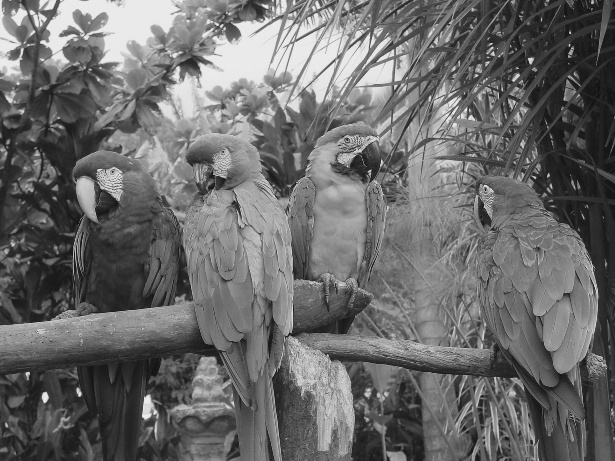
\includegraphics[width=\textwidth]{Y.jpg}
        \caption{$Y$ channel}
        \label{fig:Y}
    \end{subfigure}
    \begin{subfigure}[b]{0.2\textwidth}
        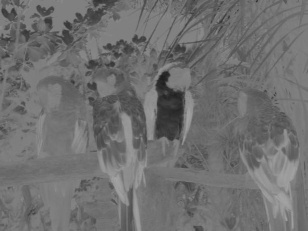
\includegraphics[width=\textwidth]{Cb.jpg}
        \caption{$C_b$ channel}
        \label{fig:Cb}
    \end{subfigure}
    \begin{subfigure}[b]{0.2\textwidth}
        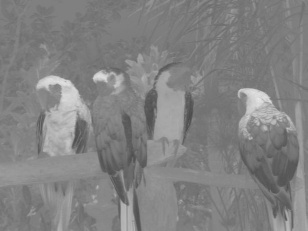
\includegraphics[width=\textwidth]{Cr.jpg}
        \caption{$C_r$ channel}
        \label{fig:Cr}
    \end{subfigure}
       \caption{$Y$, $C_b$ and $C_r$ channels}
       \label{fig:YCbCr}
\end{figure}

\subsection{Alternative downsampling algorithms}
The implemented downsampling kernels encode the image by selecting a sample pixel out of a window with a specific size. This downsampling scheme may result in aliasing artifacts \cite{Article5}. Fang et al. propose an alternative downsampling scheme based on edge detection. The edge information is used to adaptively determine sampling direction and an adaptive filter is used to preserve shape details while avoiding aliasing \cite{Article5}. This downsampling algorithm improves the resolution compared to traditional downsampling techniques, however, its implementation is much more complex.  

%------------------------------------------------------------------------
\section{Upsampling Kernels}
The purpose of the decoder is to use the downsampled $Y$, $C_b$, and $C_r$ channels to recover the original image (to its best ability). This can be accomplished by using an upsampling algorithm to resample the individual channels and finally converting the upsampled channels back to the RGB space to be displayed. 

\subsection{Implementation of upsampling kernels}
The upsampling kernels implement a bilinear interpolation algorithm to resample each of the $Y$, $C_b$ and $C_r$ channels back to the original image's size. The \verb|ycbcr2rgb| method shown in \cref{color-transforms} is then called to convert the resampled $Y$, $C_b$ and $C_r$ channels to the RGB space. At this point, the reconstructed image can be displayed.
{\footnotesize
\begin{verbatim}
def decode(self, Y, Cb, Cr):
    size = self.original_image.shape[:2]

    # Upsample Y by a factor of 2
    Y = self.bilinear(Y, size)

    # Upsample Cb and Cr by a factor of 4
    Cb = self.bilinear(Cb, size)
    Cr = self.bilinear(Cr, size)

    R, G, B = self.ycbcr2rgb(Y, Cb, Cr)

    self.image = cv2.merge((B, G, R))
    return cv2.merge((B, G, R))
\end{verbatim}
}
The code above shows the implementation of the decoder; it takes the downsampled $Y$, $C_b$ and $C_r$ channels as parameters and returns the image in the RGB color space.


\subsection{Bilinear Interpolation}
Bilinear interpolation uses the weighted average of the 4 nearest pixels to compute or interpolate the value of the missing pixel. As the name implies, bilinear interpolation involves interpolating in a single, linear direction once and then interpolating in the other direction. 

The first step in bilinear interpolation is to define the interval of every new pixel in both the $x$ and $y$ dimensions. This is achieved by dividing the current height or width by the height or width of the new image (desired size). The resulting ratio is the interval at which every new pixel is interpolated. The next step is to interpolate in each direction by finding the 4 surrounding pixels and their respective weights. The weight is based on the the distance in a single direction between the interpolated pixel and the nearest pixel. This algorithm can be implemented as follows:
{\footnotesize
\begin{verbatim}
def bilinear(self, image, dimension):
    height, width = image.shape[:2]
    new_height, new_width = dimension

    upsampled = np.empty([new_height, new_width])

    x_ratio = float((width - 1) / (new_width - 1))
    y_ratio = float((height - 1) / (new_height - 1))

    for i in range(new_height):
        for j in range(new_width):
            x1 = math.floor(x_ratio * j)
            y1 = math.floor(y_ratio * i)
            x2 = math.ceil(x_ratio * j)
            y2 = math.ceil(y_ratio * i)

            p11 = image[y1, x1]
            p12 = image[y1, x2]
            p21 = image[y2, x1]
            p22 = image[y2, x2]

            x_weight = (x_ratio * j) - x1
            y_weight = (y_ratio * i) - y1

            pixel = p11 * (1 - x_weight) * \ 
            (1 - y_weight) + \
            p12 * x_weight * (1 - y_weight) + \
            p21 * y_weight * (1 - x_weight) + \
            p22 * x_weight * y_weight

            upsampled[i, j] = pixel.astype(np.uint8)
    return upsampled
\end{verbatim}
}
Note that the computational complexity of this algorithm is $O(m\times n)$, where $m$ and $n$ are the height and width of the resampled image, respectively. As the image grows large, the time it would take to perform this computation would increase significantly.
\subsection{Alternative upsampling algorithms}
Other interpolation algorithms include nearest neighbour and bicubic interpolation. Nearest neighbour simply takes a single pixel in a window and copies that pixel to resize the image. Although this algorithm has linear time complexity, the quality of the resultant image would be unsatisfactory for this application. Bicubic interpolation is similar to bilinear in that it finds the weighted average of surrounding pixels. While bilinear only computes 4 parameters corresponding to 4 surrounding pixels, bicubic interpolation uses 16 parameters, making it slower but producing a better quality image.
%------------------------------------------------------------------------
\section{Results and Discussion}
\cref{fig:upampled} shows the reconstructed image after going through the encoding-decoding pipeline: converting to $YC_bC_r$ color space, downsampling each channel, upsampling each channel, and converting back to RGB color space. There are slight distortions and artifacts in the reconstructed image, especially near edges and textured areas such as the feathers and under the eyes of the parrots. These artifacts are due to calculations in the upsampling kernels using bilinear interpolation.
\begin{figure*}
  \centering
  \begin{subfigure}{0.72\linewidth}
    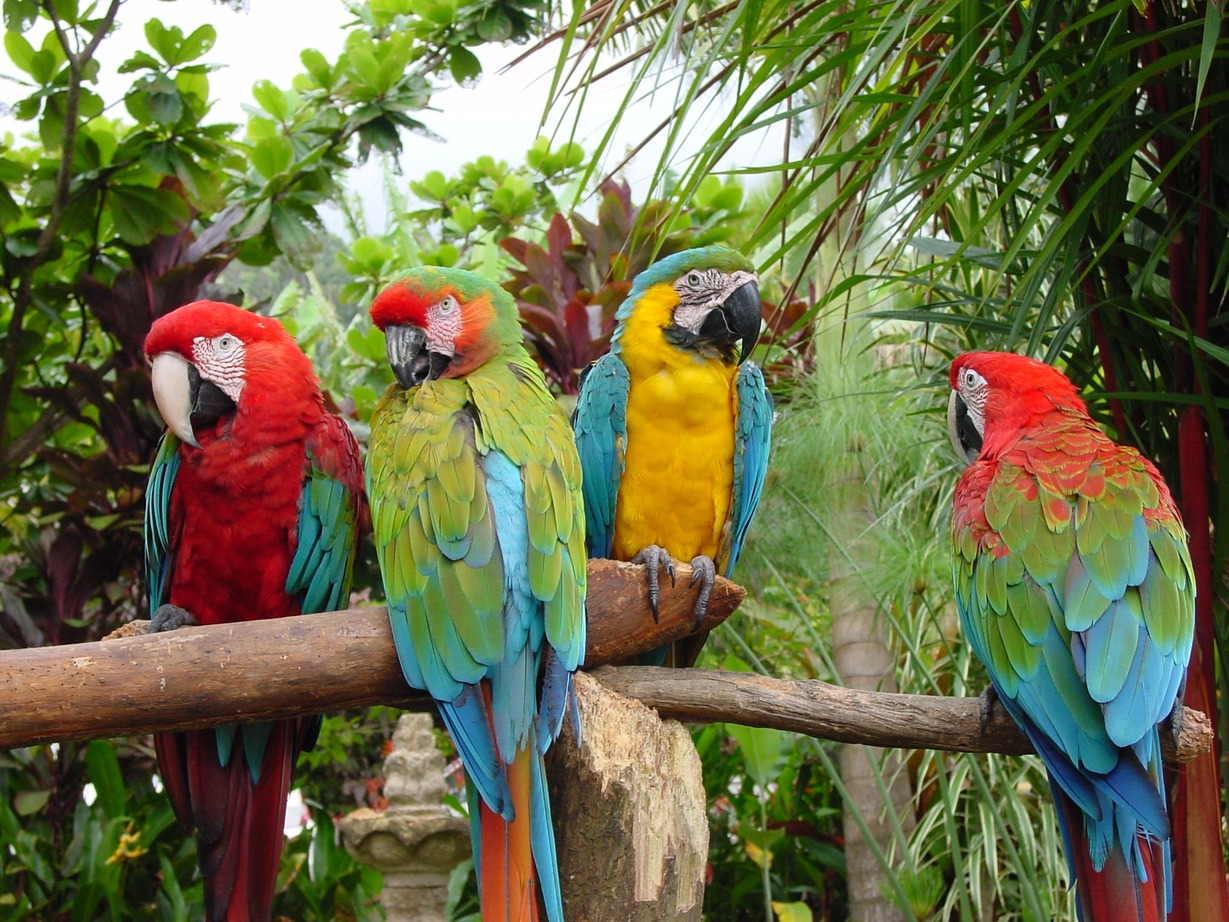
\includegraphics[width=\textwidth]{birds.jpg}
    \caption{Original image}
    \label{fig:original}
  \end{subfigure}
  \vfill
  \begin{subfigure}{0.72\linewidth}
    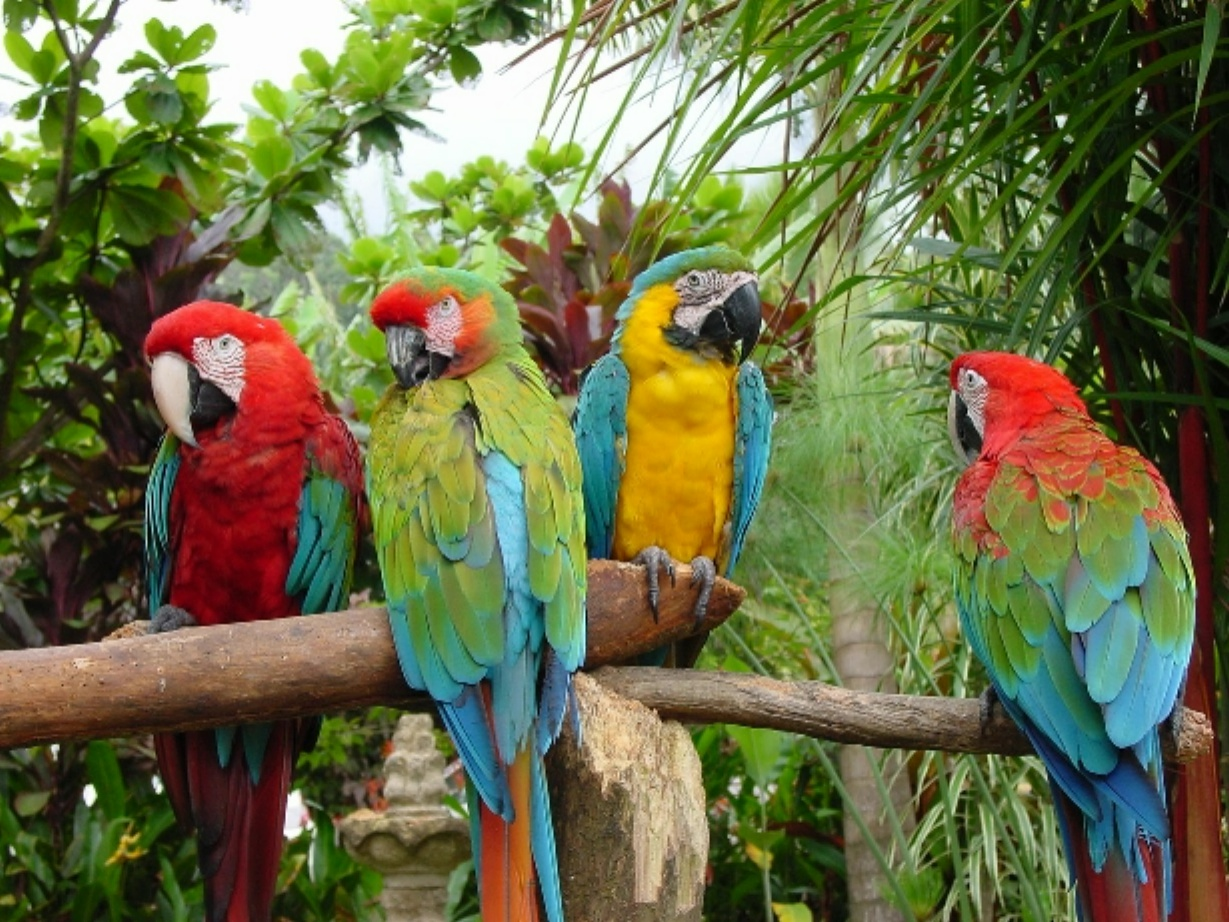
\includegraphics[width=\textwidth]{upsampled.jpg}
    \caption{Original image and image after encoding and decoding}
    \label{fig:upampled}
  \end{subfigure}
  \caption{Original image and image after encoding and decoding}
  \label{fig:birds}
\end{figure*}

\subsection{PSNR Calculation}
PSNR, or peak signal-to-noise ratio is a metric commonly used to quantify the quality of a reconstructed image. It is given by the following relation:
\begin{equation}
    PSNR = 10log_{10}(\frac{255^2}{MSE})
\end{equation}
Where $MSE$ is the mean squared error and is the mean of the difference between the original image and the reconstructed image, squared.

In the code, PSNR was calculated as follows:
{\footnotesize
\begin{verbatim}
def get_psnr(self):
    mse = np.mean(
        (self.original_image - self.image)** 2
    )
    return 10 * math.log10(255.0**2 / mse)
\end{verbatim}}
Note that if the original and reconstructed image are the same, then PSNR is infinite.

For the reconstructed image in \cref{fig:birds}, the PSNR is \textbf{32.667819dB}.
%------------------------------------------------------------------------
\section{Conclusion}
This project implemented a lossy compression method using forward and inverse color transforms for RGB and $YC_bC_r$, simple downsampling, and upsampling using bilinear interpolation. The program (Python script) implements the encoder and decoder and reports back PSNR of the reconstructed image. 

{\small
\bibliographystyle{ieee_fullname}
\bibliography{bib}
}

\end{document}
